\paragraph{Оценка частоты с использованием АР-модели}

Для использования АР-модели в задаче оценки частоты сигнала в сетях с широкополосными сигналами, необходимо знать фазу ПСП.
Для оценки фазы ПСП в данной работе используется алгоритм Delay and Multiply Approach, который предложен в \cite{tsui, lin_dma}.
Данный алгоритм позволяет свести перебор в двух областях: частота и фаза ПСП к перебору в одной - фаза ПСП.
Стоит отметить недостаток алгоритма DMA – невозможность использовать в слабых сигналах, так как алгоритм увеличивает уровень шума
в процессе детектирования.

Схематично приемник с использованием АР-модели для оценки частоты представлен на рисунке \ref{pic:ar_cdma_scheme}.
Точность оценки частоты АР-методом позволяет использовать значение оценки непосредственно в качестве начального значения для запуска ФАПЧ.

\begin{figure}[H]
	\center\scalebox{1}{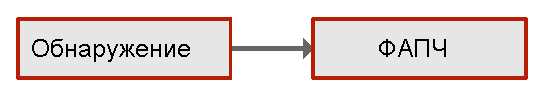
\includegraphics[width=1\linewidth]{ar_scheme.eps}}
	\caption{Схема приемника на основе АР-модели}
	\label{pic:ar_cdma_scheme}
\end{figure}

Разрешающая способность оценки частоты и использованием АР-метода зависит от величины ОСШ. В данной работе рассматривается
АР-модель 2 порядка с одной гармонической компонентой, тем не менее представляется возможным использовать приближенную
формулу Марпла \cite{kay_ar_book, marpl_book} для оценки разрешающей способности:

\begin{equation}
	\label{eq:ar_cdma_marple_eq}
	F = \frac{1.03}{Tp[SNR(p+1)]^{0.31}}
\end{equation}
где ${F}$ – разрешение в герцах, ${Т}$ - интервал отсчетов в секундах, p-максимальное значение временного сдвига для АКФ
последовательности, а ${SNR}$ - ОСШ выраженное в линейных единицах. В задаче оценке частоты в ПСП-модулированном сигнале ${p=2}$.
График зависимости точности от ОСШ представлен на рисунке \ref{pic:cdma_ar_marple_eq}.

\begin{figure}[H]
	\center\scalebox{0.8}{\includegraphics[width=1\linewidth]{marple_eq.eps}}
	\caption{Оценка зависимость точность оценки частоты от ОСШ по ф. Марпла}
	\label{pic:cdma_ar_marple_eq}
\end{figure}
